\chapter{Introduction}
\label{cha:intro}

In the first two parts of this chapter a brief overview will explain the most known databases technologies while in the last part NoSQL databases will be introduced through the descrption of the most famous implementations from which many others derive.


\section{Discovery of NoSQL technologies}
\label{sec:context}

Commonly students have their first encounters with database technologies during their studies in high school or bachelor degree and, to better understand all the fundamentals concepts, they are taught the basic principles of relational databases.
It i’s the most common choice of every school teaching the very foundation of Databases to make students understand the the meaning of \textit{CRUD operations, relations, consistency, redundancy} \footnote{https://en.wikipedia.org/wiki/Create,\_read,\_update\_and\_delete}, etc... and how to correctly set up the entities of their systems following proven patterns and constraints.
Detaching from well-known developing habits is not always so simple, but it is necessary to understand why big companies such as Facebook decided to invest money in developing their own database solution, Cassandra, instead of using an existing relational database.
It is important to know that there are many different ways to build a database, some are better than others in certain use cases. Nowadays, an huge amount of data are spread around the world everyday through the Web and it needs to be stored and retriewed quickly to save companies' money and give the users a perfect feeling of resposivity\cite{ictbusiness}.
But let’s start from the beginning to get an overview of a technology we rely on every day, even without being aware of its presence in every single application we use.


\section{Databases}
\label{sec:problem}

A Database is an organized collection of data even though we often use the term to refer to the entire database system. The Database Management System, or DBMS, is the name of the entire system that handles data, transactions, relations and eventually problems.
The term DBMS has been replaced by RDBMS in the common language, that stands for Relational Database Management Systems, since for decades the relational model has been a standard for data storage.


\subsection{Relational Databases}
\label{sec:description}

Probably the most popular and for many years also most used model, a relational database is composed by tables representing entities (users, customers, courses...) where each column represents a field or attribute and each row represents a record.
Tables can have relations each other with the use of foreign keys, and each table has a primary key that is unique on each record.
It’s fundamental for a good design of a relational database that its schema is in \textit{Normal Form}, following three main steps:
\begin{itemize}
	\item \textit{First Normal Form} : Eliminating groups of repeated data and creating a table for each group of related data identified with a primary key.
	\item \textit{Second Normal Form} : Moving all identical set of values for multiple records to a new table and using a foreing key to link them.
	\item \textit{Third Normal Form} : Removing all fields not dependent on the primary key or, if they are necesary, putting them into another table.
\end{itemize}
Apart from Normal Form, to ensure that a relational database guarantees the reliability of its transactions it must ensure ACID\footnote{http://www.service-architecture.com/articles/database/acid\_properties.html} properties:
\begin{itemize}
	\item \textit{Atomicity} : A transaction must be completed in all of its parts or none.
	\item \textit{Consistency} : Transactions preserve the integrity of the database and they do not leave the database in an invalid state after occurring.
	\item \textit{Isolation} : Transactions must be isolated to guarantee that any inconsistency does not affect data of other transactions.
	\item \textit{Duraibility} : Completed transactions make changes that must be durable.
\end{itemize}
The most famous relational databases follow SQL syntax that stands for Structured Query Language and is a standard since 1986.
Among this category, the most famous and used are MySQL, PostgreSQL, Microsoft SQL Service, Oracle Database.
\subsection{Navigational Databases}
The first generation of databases used pointers from one record to another to “navigate” the database and that’s why they were called Navigational databases.
The fundamental problem of this kind of database was that the user needed to know the physical structure of the database to query data from it. The only way to add an extra field was achieved only by rebuilding the storage scheme.
In addition, the absence of a standardisation among vendors made those databases disappear quickly in favour of more functional choices

\subsection{Object-oriented Databases}
In the long story of the database evolution, object-oriented databases helped developing the communication between databases and programming languages, but they failed due to their bounds to a specific programming language. They offered advanced features like inheritance and polymorphism and could support a large number of data types.
What is left of their inheritance in the aftermath is the implementation of drivers and bindings between databases and programming language.
NoSQL technologies are a perfect example of the evolution of the idea of object-oriented databases.

\subsection{NoSQL Databases}
The last generation of databases is called NoSQL because of its detachment from the classic relational model in terms of schema and their use of query languages different  than SQL.
They  aim to great performance and scalability, to support the increasing need of those applications that daily transfers huge amounts of data.
Since the category is itself generic, and new different implementations are release every year, they can be broadly divided in those sub-categories:
\begin{itemize}
	\item \textit{Graph databases} : as foundation of this kind of databases there is the graph theory and the concept of nodes and edges. Each node corresponds to an entity and edges correspond to relations between them. They use an index-free adjacency that grants each element a pointer to its adjacent element and does not require the full indexing of the database.
	\item \textit{Key-value stores} : thanks to simple concepte of a key assigned to each value, similarly to has-tables, the model of those databases usually grants higher performance. It is even possible, depending on the database implementation, that a key could be bound to an entire collection of values.
	\item \textit{Document stores} : this is the family which MongoDB belongs and they work around the concept “Document”. Documents are records and they are stored into tables called collections. Usually collections don’t require the same number of fields, so there could be different versions of the same document inside a collection. A great advantage of this model is the ease of data access and manipulation.
\end{itemize}
The core aspect of theri implementation is that they have no predefined schema, in addition most of them does not require their records to have the same number of fields if not enforced, also called Dynamic Schema \footnote{http://blog.rdx.com/is-nosql-the-natural-progression-of-database-technology-0}.
They support to replication of the primary server on many other servers, like MongoDB’s ReplicaSet, and this provides reliability in case of failover of one of the nodes granting no data loss in production applications. Servers execute same transactions and keep their data synchronized to eliminate any errors, and they usually write a backup copy or a snapshot of the data after any operation. As is it possible to imagine, this multi-node architecture cannot fully guarantee the respect of ACID properties and might sometimes present synchronization issues with the possible result of a secondary node becoming primary with partially outdated data.
The absence of constraints on the schema allows query to be executed faster withput the need of expensive \textit{join} operations on the collections, but when it comes to execute complex queries NoSQL databases performance fall if they are not well configured.
It is then important to provide a good configuration of the architecture in order make the most of the strengths of those databases.




\subsection{The CAP Theorem}
This theorem, also named Brewer's theorem after the first computer scientist that stated it, states that a distributed computer system cannot simoultaneously provide more than two of the following guarantess: \textit{Consistency\footnote {Every read receives the most recent write or an error}, Availability \footnote{Every requests receives a response, but with no guarantes that it contain the most recent write}, Partition tolerance \footnote{The systems keeps operating despite the delay (or drop) of an arbitrary number of messages }}.
RDBMS for examples, designed with traditional ACID guarantees, choose Consistency and Availability and this is why they have a weak Partition tolerance.
NoSQL databases on the other side are divided in those who prefer Consistency and Partition Tolerance and those who choose Partition Tolerance and Availability.
\begin{figure}[H]
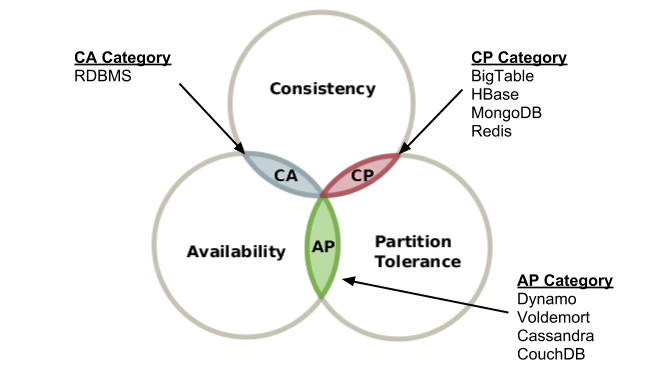
\includegraphics[scale=0.5]{cap-theorem.png}
\centering
\caption{Some famous databases partitoned following the CAP theorem.}
\end{figure}



\section {NoSQL: a brief panoramic over the actual situation}
NoSQL databases area literally spreading around, with many companies and insitutes implementing their own custom version so it would be impossible to describe them all. 
Most of them are new implementations of the pioneers who brought this innovating technology to the market less than 10 years ago, that are briefly described in the following part.

\subsection{MongoDB}
\textsc{MongoDB} is a document-oriented DBMS that uses a JSON-style documents called BSON, making data integration from certain kind of applications easier and faster.
Originally developed as a component of a bigger software, it then became open source in 2009 under the supervision of MongoDB Inc. company.
It offers support for many programming languages such as Java, C++, Python and many others and it’s being used as backed from a large number of web sites and services like eBay, Foursquare, NYTimes among the others.
As db-engines.com reports, it is the most popular NoSQL database now.


\subsection{Google Big Table}
\textsc{Big Table} is the proprietary database system of Google, developed back in 2004 and build on Google File System \footnote{https://en.wikipedia.org/wiki/Google\_File\_System}. It shares the characteristics both of row-oriented databases and column-oriented databases. Google decided to develop its own database with the purpose of scalability and better control over performance: in fact it’s designed to support a data-load of petabytes over thousands of machines.
Big Table supports many Google applications such as Reader, Maps, Books, Earth, Gmail and even YouTube.
Google announced a new version called Google Cloud Bigtable\footnote{https://cloud.google.com/bigtable}, actually in beta, that will be distributed as public version of Big Table.

\subsection{Apache Cassandra}
Another open-source project is \textsc{http://cassandra.apache.org/} \footnote{apache cassandra}, developed at Facebook in 2007 to improve the research of the internal mail system and then entered in the Incubator project from Apache in 2008 where it begun its growth as DBMS.
Like Big Tables it offers a key-value storage structure with eventual consistency. Each keys correspond to a value and all the values are grouped in families of columns. Families are defined when the database is created and Cassandra adopts an hybrid approach between DBMS oriented to columns and memorization oriented to rows.
Other famous sites than Facebook that uses Cassandra are Twitter and Digg, and many benchmark tests, in terms of performance and scalability confirms Cassandra as the best NoSQL database in the current scenario.

\subsection{Amazon DynamoDB}
\textit{Amazon DynamoDB} \footnote{https://aws.amazon.com/it/dynamodb} is the proprietary database system of Amazon available for developers since 2012, build on the model of Dynamo but with a different implementation and offered as a part of the Amazon Web Services \footnote{amazon web services} portfolio. The particularity is that DynamoDB allows developer to purchase a service based on the desired throughput rather than the storage, that will be increased by the administrators of the system if needed.
Many programming languages have a DynamoDB binding, including Java, Node.js, Python, Perl and C\#.
Most of the Amazon services uses DynamoDB as storage system.


